\documentclass[a4paper,10pt]{article}
\usepackage[top=2cm, bottom=2cm, left=3cm , right=3cm]{geometry}
%\usepackage{hyperref}
\usepackage{fancyhdr}
\pagestyle{fancy}
\usepackage{subfig}
\usepackage{graphicx}
\usepackage{amsfonts}
\usepackage{stmaryrd}
\usepackage{multicol}
%\documentclass[a4paper,10pt]{scrartcl}

\usepackage[utf8]{inputenc}
\usepackage{wasysym}

\title{}
\author{BENJELLOUN Hicham}
\date{}

\pdfinfo{%
  /Title    ()
  /Author   ()
  /Creator  ()
  /Producer ()
  /Subject  ()
  /Keywords ()
}
\renewcommand{\contentsname}{Table des matières}
\begin{document}
\lhead{BENJELLOUN Hicham - 1A INFO}
\rhead{Rendu le 16/01/2013}
\begin{figure}[!h]
 \centering
 
\includegraphics[scale=0.6]{logo.jpg}
\end{figure}

\begin{center}
 {\Large \textbf{Fondements de l'Informatique}} \\
 \textit{Projet - Réduction de couleurs}\\
\end{center}
\noindent
Encadrant de TP : BRUN Luc

\tableofcontents

\section{Introduction}
L'objectif de ce projet est, étant donné une image possedant potentiellement $256^3$ couleurs différentes, de la représenter à l'aide d'un nombre fixe $K<256^3$ couleurs.
Pour cela, on utilisera un algorithme de \textbf{quantification par popularité} qui consiste à remplacer chaque couleur par la couleur de plus haute fréquence qui lui est la plus proche.
\newline
\newline
Ce travail présente brièvement\footnote{La description des fonctions et leurs commentaires étant présents dans les sources.} l'ensemble des structures et fonctions créees dans ce but, en détaille les algorithmes\footnote{Décrits en énoncé} ou en propose des alternatives ou optimisations.
\section{Organisation du répertoire de travail}


\section{Calcul d'histogramme couleur}
Un histogramme couleur d'une image $I$ permet d'associer une couleur $(R,G,B)$ à sa fréquence d'apparition $f$ dans $I$.
\newline
Un représentation par un tableau $256\times256\times256$ prendrait trop de place en mémoire. Par ailleurs, une représentation de $\cal{H}$ par une liste de liste de liste permettrait d'optimiser spatialement son occupation mémoire, mais augmenterait
significativement la complexité des algorithmes de construction et de traitement de l'histogramme du fait des parcours de liste.
\newline
Un bon compromis serait donc de représenter $\cal{H}$ par un tableau à deux dimensions, donc chaque élément $(R,G)$ pointe vers une liste contenant les valeurs de $B$.

\subsection{Manipulation de listes}
L'algorithme d'insertion d'une cellule dans une liste, de complexité linéaire à été vu en cours. La seule différence est que lorqu'on trouve la cellule, on augmente simplement son champ \verb freq  .

\subsection{Construction, initialisation et destruction de l'histogramme}
\subsubsection{Construction de l'histogramme} 
\begin{verbatim}
histo create_histo() 
\end{verbatim}
Alloue un tableau à deux dimensions en mémoire et initialise chaque cellule à \verb NULL et le renvoie en sortie.
\subsubsection{Initialisation à partir d'une image}
\begin{verbatim}
void init_histo(histo,image)
\end{verbatim}
Initialise l'histogramme à partir d'une image donnée.
\subsubsection{Destruction}
\begin{verbatim}
void delete_histo(histo)
\end{verbatim}
Libère l'histogramme de la mémoire.

\subsection{Interrogation de l'histogramme}

Une fois l'histogramme $\cal{H}$ crée, on a besoin d'un outil qui nous permet de parcourir facilement l'ensemble des couleurs présentes dans l'histogramme : on va utiliser un itérateur, qui pointe sur un cellule
et qu'on pourra facilement modifier pour qu'il pointe sur la couleur suivante.
\newline
\newline
On le définit comme étant une structure privée du module \verb histo  \newline
\noindent
Néanmoins, on peut constater qu'il pourrait être utile de pouvoir utiliser cette structure en dehors du module, comme par exemple dans le module quantification. En effet, lorsque l'on compare la fréquence
de la couleur contenu dans la cellule pointée par l'itérateur pour savoir s'il faut l'insérer dans la liste des $K$ couleurs de plus haute fréquence, on fait appel à une fonction qui nous donne la fréquence
par un parcours de la liste $(R,G)$ alors que cette même fréquence est contenue dans la cellule pointée directement par l'itérateur : il faudrait donc plutôt créer une fonction \verb give_freq_histo_iter()  plutôt
qui renvoie directement le champs \verb freq  de la cellule pointée par l'itérateur.

\subsubsection{Récupération de la fréquence d'une couleur}
\begin{verbatim}
int give_freq_histo(histo h,int R,int G,int B)
\end{verbatim}
Renvoie la fréquence associée à la couleur $(R,G,B)$ à partir de l'histogramme $h$.

\subsubsection{Création et positionnement de l'itérateur}
\begin{verbatim}
histo_iter create_histo_iter(histo h)
\end{verbatim}
Alloue en mémoire l'itérateur et le place à la première entrée non nulle de l'histogramme $h$.

\subsubsection{Repositionnement de l'itérateur}
\begin{verbatim}
histo_iter start_histo_iter(histo h)
\end{verbatim}
Alloue en mémoire l'itérateur et le place à la première entrée non nulle de l'histogramme $h$.

\subsubsection{Couleur de l'itérateur}
\begin{verbatim}
void give_color_histo_iter(histo_iter iter, int *c)
\end{verbatim}
Copie la couleur de l'itérateur \verb iter  dans le tableau pointé par \verb c  .

\subsubsection{Destruction de l'itérateur}
\begin{verbatim}
void delete_histo_iter(histo_iter)
\end{verbatim}
Désallour la mémoire associée à un itérateur.

\section{Implémentation de ppmhist}

Le programme \verb ppmhist  utilise le travail réalisé précédemment pour afficher les différentes couleurs de l'image ainsi que leur luminosité et leur fréquence d'apparition.
Il se structure suivant les étapes suivantes :
\begin{itemize}
\item[ \textbf{E1.}] Chargement de l'image
\item[ \textbf{E2.}] Positionnement du pointeur courant au début de l'image

\item[ \textbf{E3.}] Création de l'histogramme
\item[ \textbf{E4.}] Initialisation de l'histogramme à partir de l'image

\item[ \textbf{E5.}] Création de l'itérateur
\item[ \textbf{E6.}] Initialisation de l'itérateur

\item[ \textbf{E7.}] Affichage de la couleur pointée (et ses caractéristiques) par l'itérateur courant
\item[ \textbf{E8.}] Passage à l'itérateur suivant
\end{itemize}

\noindent Repeter E7,E8 Tant Que l'itérateur courant est non nul.

\section{Quantification par popularité}

Pour cette partie, on définit préalablement une nouvelle structure de liste dont chaque cellule contient un tableau codant une couleur $(R,G,B)$, la fréquence correspondante et un pointeur
sur la cellule suivante.

\subsubsection{Quantification}
\begin{verbatim}
void quantification(histo h,int *tab,int K)
\end{verbatim}

\begin{itemize}
 \item [\textbf{E1.}] On initialise une liste de longueur $K$ contenant la liste des $K$ premières couleurs de l'image.  
 \item [\textbf{E2.}] On ajoute chaque cellule restante de l'histogramme parcouru à l'aide de l'itérateur à la liste si cette cellule est de fréquence plus grande que la couleur pointée par la tête de la liste 
 (qui est par construction de fréquence minimale car la liste est triée par ordre croissant). À la fin de cette étape, on dispose dans une liste des $K$ couleurs de plus haute fréquence.
 \item [\textbf{E3.}] On convertit cette liste\footnote{La structure de liste permet temporairement de pouvoir faire des insertions sans avoir à réaliser de décalage} en tableau de taille $3\times K$.
\end{itemize}

\subsubsection{Couleur la plus proche}
\begin{verbatim}
closest_color(int* tab,int K,int R,int G,int B,int*output)
\end{verbatim}
Pour une couleur $(R,G,B)$ donnée, renvoie la couleur $(R',G',B')$ appartenant au tableau \verb tab  la plus proche de $(R,G,B)$, \textit{i.e} celle minimisant la quantité $\sqrt{(R'-R)^2+(G'-G)^2+(B'-B)^2}$
\footnote{Ou son carré, ce qui revient au même et qui est moins coûteux en temps de calcul.}

Il s'agit d'un simple parcours d'un tableau de longueur $3K$, donc en complexité linéaire. On peut améliorer cette complexité en réalisant une recherche par dichotomie.

\subsubsection{Mapping}
\begin{verbatim}
void mapping(image input,image output,int* tab,int K)
\end{verbatim}
Cette fonction parcours simplement l'image d'entrée et modifie la couleur de chaque pixel par celle qui lui est la plus proche (voir fonction précédente) dans la liste des $K$ couleurs de plus haute fréquence.

\section{Quelques résultats}

\begin{figure}[!htp]
  \centering
  \subfloat[Image d'origine]{\label{fig:edge-a}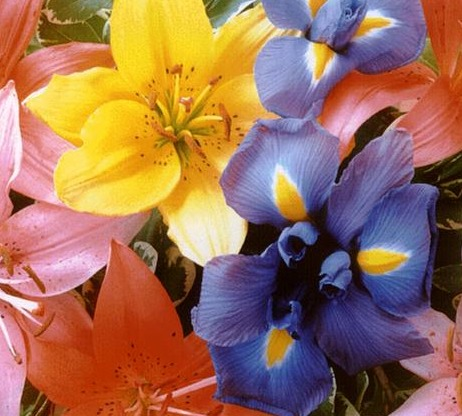
\includegraphics[scale=0.35]{original.jpg}}                
  \subfloat[1024 couleurs]{\label{c1024}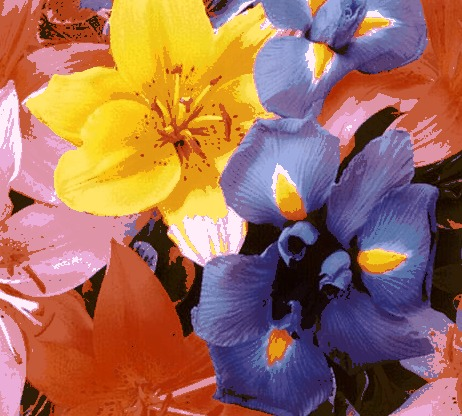
\includegraphics[scale=0.35]{c1024.jpg}}
  \subfloat[128 couleurs]{\label{c128}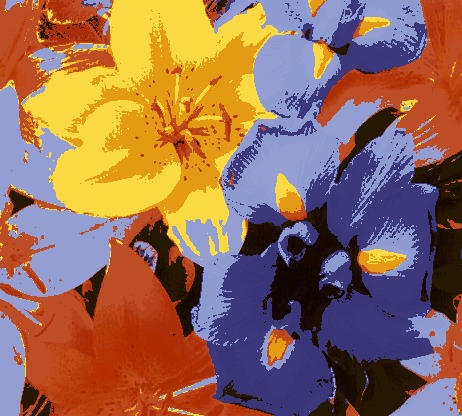
\includegraphics[scale=0.35]{c128.jpg}}
  \caption{Tests pour l'image \texttt{fleurs.ppm} }
  \label{fig:contour}
\end{figure}

\begin{figure}[!htp]
  \centering
  \subfloat[Image d'origine]{\label{fig:edge-a}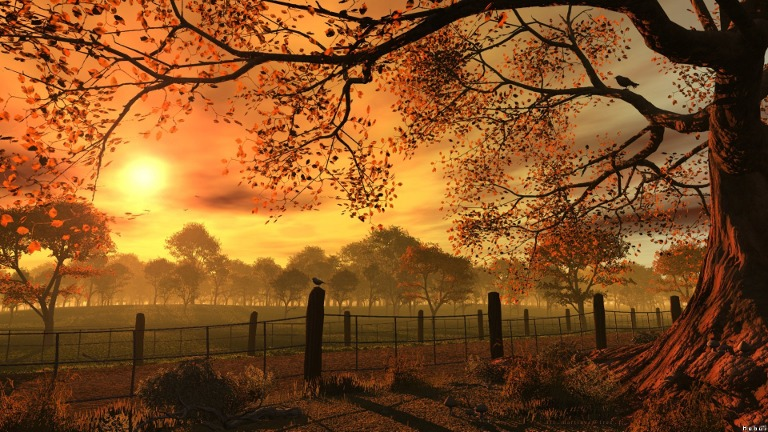
\includegraphics[scale=0.30]{aaa.jpg}}                
  \subfloat[1024 couleurs]{\label{c1024}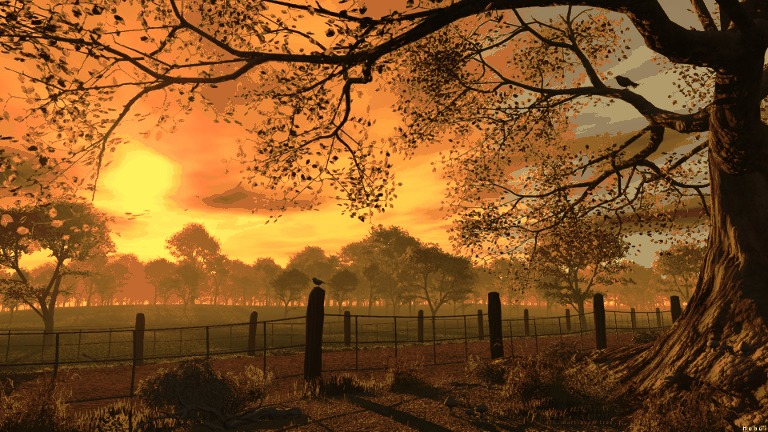
\includegraphics[scale=0.30]{d1024.jpg}}
  \label{fig:contour}
\end{figure}


\begin{figure}[!h]
  \centering
  \subfloat[128 couleurs]{\label{c128}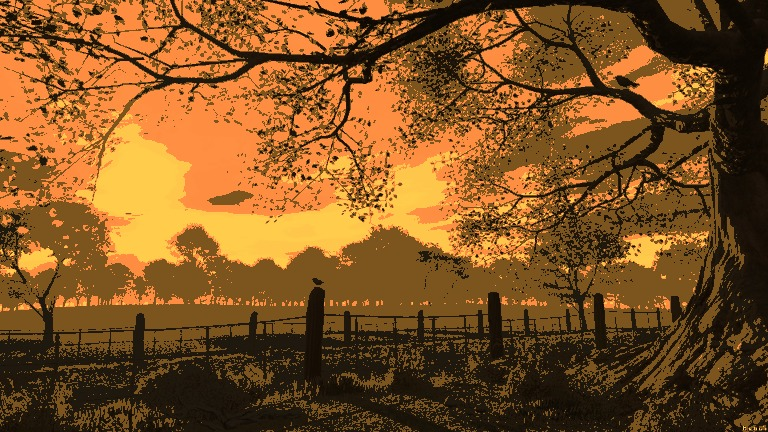
\includegraphics[scale=0.30]{d128.jpg}}
  \label{fig:contour}
\end{figure}

\end{document}